\documentclass[10pt]{article}
\usepackage[a4paper,margin=1.3cm,top=1.1cm,bottom=1.1cm]{geometry}
\usepackage{booktabs}
\usepackage{array}
\usepackage{multirow}
\usepackage{amsmath}
\usepackage{xcolor}
\usepackage{titlesec}
\usepackage{enumitem}
\usepackage{tikz}
\usetikzlibrary{arrows.meta,positioning}
\usepackage{pgfplots}
\pgfplotsset{compat=1.18}
\pagestyle{empty}

\titleformat{\section}{\normalfont\large\bfseries}{\thesection}{0.5em}{}
\titlespacing*{\section}{0pt}{5pt}{2pt}
\titleformat{\subsection}{\normalfont\bfseries}{\thesubsection}{0.5em}{}
\titlespacing*{\subsection}{0pt}{4pt}{1pt}

\definecolor{hl}{HTML}{0B5394}

\setlength{\parindent}{0pt}
\setlength{\parskip}{1pt}
\setlength{\tabcolsep}{4.5pt}

\begin{document}

% ============================= PAGE 1 =============================
\begin{center}
{\LARGE\bfseries A Domain-Agnostic Reconstruction Pipeline for GNSS Spoofing}\\[2pt]
{\large Method Overview: Aviation \& Maritime}
\end{center}
\vspace{2pt}

When an aircraft or vessel's satellite-navigation signal is spoofed,
surveillance operators must discard its broadcast position yet keep
tracking it. Existing trajectory predictors are trained for a single
transport domain and must be rebuilt for each new one. \textbf{TrajRAG
factors the problem into a shared, training-free engine and a thin,
domain-specific adapter}, so that porting it from aircraft to ships requires
no model training at all -- only a prompt template, a memory index, a
trusted non-satellite signal, and a short calibration run.

\section*{Shared Engine + Domain Adapter}

\begin{center}
\resizebox{\linewidth}{!}{%
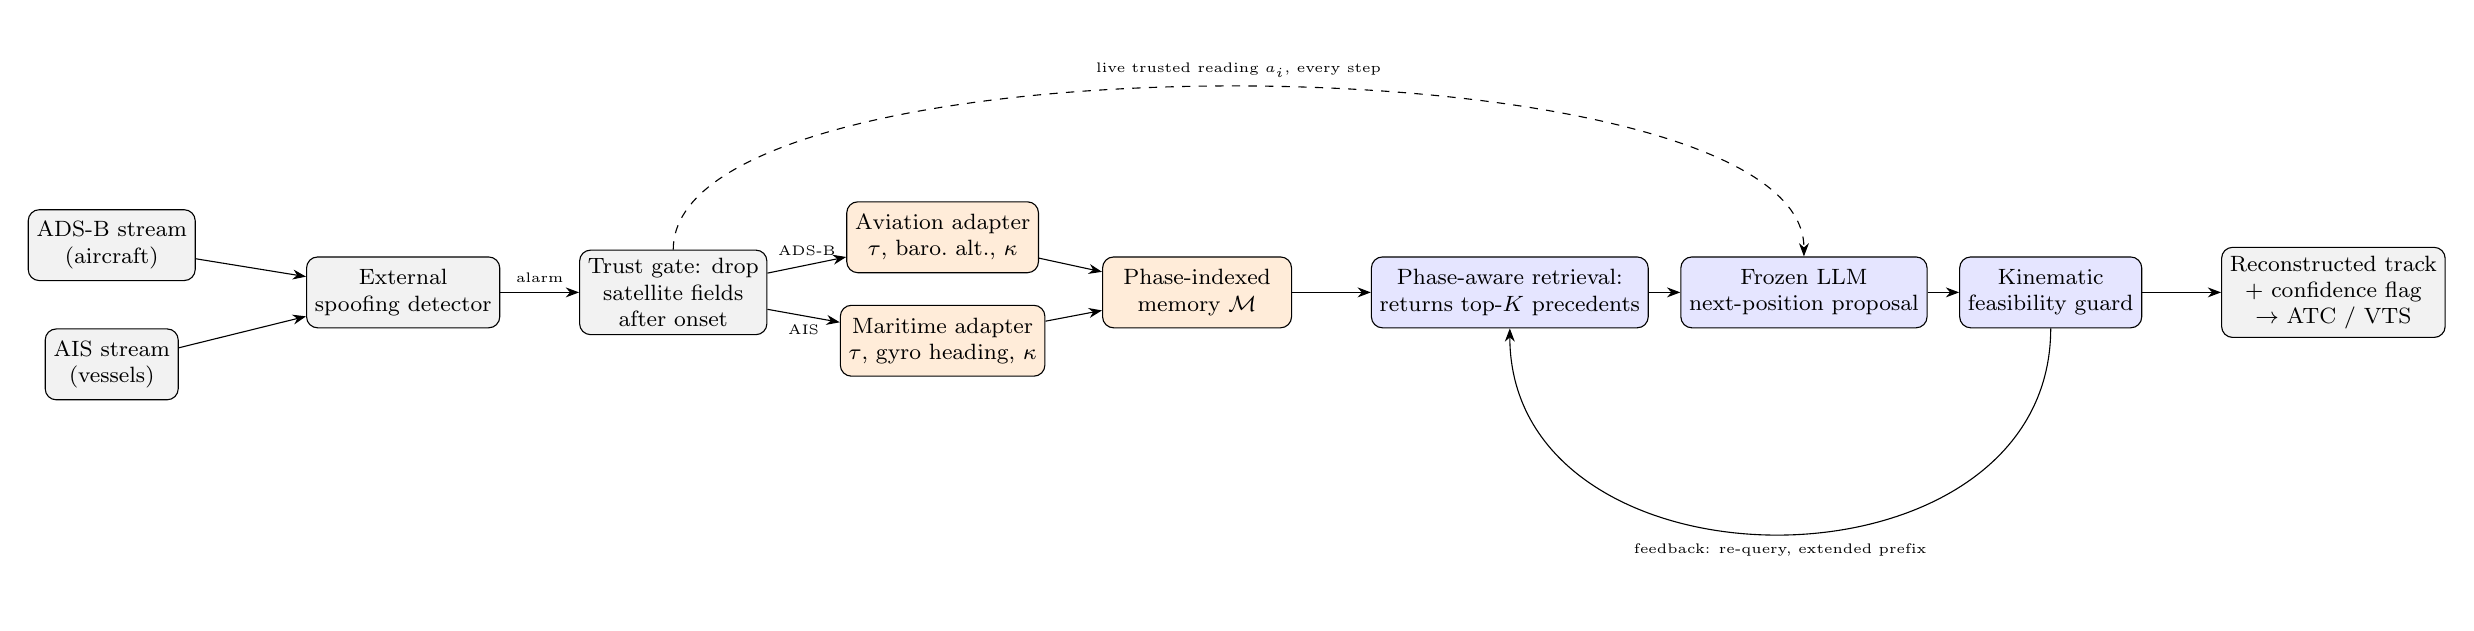
\begin{tikzpicture}[
  node distance=10mm and 8mm,
  box/.style={draw, rounded corners, align=center, minimum height=9mm, font=\footnotesize, inner sep=3pt},
  adapter/.style={box, fill=orange!15},
  engine/.style={box, fill=blue!10},
  io/.style={box, fill=gray!10},
  >=Stealth
]
\node[io] (adsb) {ADS-B stream\\(aircraft)};
\node[io, below=6mm of adsb] (ais) {AIS stream\\(vessels)};
\node[io, right=14mm of adsb, yshift=-6mm] (detector) {External\\spoofing detector};
\node[io, right=10mm of detector] (gate) {Trust gate: drop\\satellite fields\\after onset};
\node[adapter, right=10mm of gate, yshift=7mm] (adaptA) {Aviation adapter\\$\tau$, baro.\ alt., $\kappa$};
\node[adapter, below=4mm of adaptA] (adaptM) {Maritime adapter\\$\tau$, gyro heading, $\kappa$};
\node[adapter, right=8mm of adaptA, yshift=-7mm, minimum width=24mm] (memory) {Phase-indexed\\memory $\mathcal{M}$};
\node[engine, right=10mm of memory, minimum width=26mm] (retrieval) {Phase-aware retrieval:\\returns top-$K$ precedents};
\node[engine, right=4mm of retrieval] (llm) {Frozen LLM\\next-position proposal};
\node[engine, right=4mm of llm] (guard) {Kinematic\\feasibility guard};
\node[io, right=10mm of guard] (out) {Reconstructed track\\+ confidence flag\\$\to$ ATC / VTS};
\draw[->] (adsb) -- (detector);
\draw[->] (ais) -- (detector);
\draw[->] (detector) -- node[above,font=\tiny]{alarm} (gate);
\draw[->] (gate) -- node[above,font=\tiny]{ADS-B} (adaptA);
\draw[->] (gate) -- node[below,font=\tiny]{AIS} (adaptM);
\draw[->] (adaptA) -- (memory);
\draw[->] (adaptM) -- (memory);
\draw[->] (memory) -- (retrieval);
\draw[->] (retrieval) -- (llm);
\draw[->] (llm) -- (guard);
\draw[->] (guard) -- (out);
\draw[->] (guard.south) to[out=270,in=270,looseness=1.3] node[below,font=\tiny]{feedback: re-query, extended prefix} (retrieval.south);
\draw[->, dashed] (gate.north) to[out=90,in=90,looseness=0.5] node[above,font=\tiny]{live trusted reading $a_i$, every step} (llm.north);
\end{tikzpicture}%
}
\end{center}
{\footnotesize Both surveillance streams share one detector, one trust gate,
one retrieval engine, one frozen LLM, and one kinematic guard. Only the
orange domain adapter (prompt template, trusted signal, kinematic constants,
and the memory built from that domain's history) changes between aircraft
and ships.}

\section*{Aviation Data vs. Maritime Data}

\begin{center}
\begin{tabular}{p{2.6cm}p{6.3cm}p{6.3cm}}
\toprule
 & \textbf{Aviation} & \textbf{Maritime} \\
\midrule
Source & FlightRadar24 (ADS-B) & NOAA Marine Cadastre (AIS, public) \\
Corridors & Paris$\to$Rome; Barcelona$\to$Munich & Houston Ship Channel; Los Angeles/Long Beach approach \\
Trajectories & 1,544 flights & 3,506 commercial vessel voyages \\
Native sampling & $\approx$120\,s & Irregular; resampled to 300\,s \\
Trusted signal & Barometric altitude (air-data system) & Gyrocompass true heading \\
Phases & Takeoff / cruise / landing & Departure / transit / arrival \\
Environmental context & Meteomatics (wind, turbulence) & Open-Meteo Marine (waves, swell, current) \\
LLM backbone & gpt-5.1, $K{=}5$ retrieved precedents & gpt-4.1, $K{=}6$ retrieved precedents \\
\bottomrule
\end{tabular}
\end{center}
\vspace{2pt}

\textbf{The adapter is the only thing that changes.} The engine, the
retrieval mechanism, the feedback loop, and the guard's functional form are
byte-identical across both domains; only the five adapter elements above
differ, and the kinematic tolerance constant is re-derived per domain from
real data rather than reused (the one thing that did \emph{not} transfer
automatically between domains).

\newpage
% ============================= PAGE 2 =============================
\begin{center}
{\LARGE\bfseries Maritime Results}\\[2pt]
{\large Houston Ship Channel \& Los Angeles/Long Beach}
\end{center}
\vspace{2pt}

TrajRAG reconstructs a vessel's trajectory during a satellite-navigation
blackout using a \emph{frozen} large language model, retrieval of similar
historical voyages, and a kinematic feasibility guard --- with \textbf{no
model training on maritime data}. We compare it against classical filters,
recurrent networks, retrieval-only baselines, modern time-series
forecasters, and AIS-ACNet, a convolutional network trained specifically on
this task and corridor. Mean Haversine error (km, lower is better).

\section*{Main Result: Houston Ship Channel}

\begin{center}
\begin{tabular}{lccc}
\toprule
\textbf{Method} & \textbf{Departure} & \textbf{Transit} & \textbf{Arrival} \\
\midrule
Kalman filter & 3.16 & 2.61 & 4.23 \\
ARIMA & 3.64 & 3.78 & 2.24 \\
LSTM & 10.44 & 7.99 & 6.42 \\
BiLSTM & 10.03 & 14.10 & 16.43 \\
Mean-Retrieval (no LLM) & 13.89 & 8.76 & 7.03 \\
Numeric-kNN & 5.53 & 3.93 & 3.17 \\
AIS-ACNet (trained on this corridor) & \textbf{1.80} & \textbf{1.66} & \textbf{1.18} \\
\textbf{TrajRAG (no training)} & 2.19 & 1.95 & 1.50 \\
\bottomrule
\end{tabular}
\end{center}
\vspace{1pt}
{\footnotesize Also evaluated: seven modern forecasters (DLinear, PatchTST,
iTransformer, Informer, Autoformer, FEDformer, TimesNet) on a shorter,
exact-fit horizon -- not directly comparable to the full-horizon methods
above; TrajRAG and AIS-ACNet beat all seven on that same matched horizon.}
\vspace{0pt}

\textbf{\textcolor{hl}{TrajRAG is statistically indistinguishable from AIS-ACNet in every
phase}} (paired Wilcoxon test, $p = 0.77$ / $0.56$ / $0.50$) despite using
no maritime training data at all. \textbf{TrajRAG significantly outperforms
every classical, recurrent, and retrieval-only baseline in every phase, in
both corridors} ($p \leq 6.5\times10^{-3}$, mostly $p<10^{-4}$) --- a
1.3--1.5$\times$ error reduction over the best classical method.

\section*{Ablation Study (Houston, matched pairs)}

\begin{center}
\begin{tabular}{lcccccc}
\toprule
\multirow{1}{*}{\textbf{Configuration}} & \multicolumn{2}{c}{\textbf{Departure}} & \multicolumn{2}{c}{\textbf{Transit}} & \multicolumn{2}{c}{\textbf{Arrival}} \\
 & Mean & $p$ & Mean & $p$ & Mean & $p$ \\
\midrule
Full pipeline & 2.56 & -- & 1.63 & -- & 1.47 & -- \\
w/o retrieval & 2.59 & 0.93 & 2.42 & \textbf{0.012} & 2.20 & \textbf{0.048} \\
w/o kinematic guard & 3.23 & 0.20 & 1.59 & 0.28 & 1.97 & 0.76 \\
w/o live heading signal & 2.60 & 0.31 & 1.47 & 0.90 & 1.78 & 0.62 \\
\bottomrule
\end{tabular}
\end{center}
\vspace{0pt}

\textbf{Retrieval is the dominant driver of accuracy}: removing it
significantly increases error in transit and arrival. \textbf{Removing the
live trusted heading signal has no significant effect in any phase} ---
retrieval and the guard, not the live signal alone, appear to be the
pipeline's main contributors.

\section*{Houston Ship Channel at a Glance}

\begin{center}
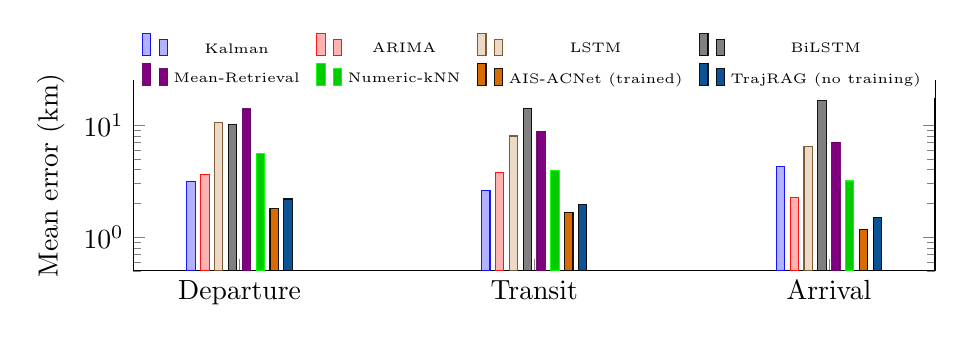
\begin{tikzpicture}
\begin{axis}[
  ybar, width=0.97\linewidth, height=4.0cm,
  ymode=log, log origin=infty,
  bar width=3.0pt,
  symbolic x coords={Departure,Transit,Arrival},
  xtick=data, tick align=inside,
  ylabel={Mean error (km)},
  ymin=0.5, ymax=25,
  enlarge x limits=0.18,
  legend style={font=\tiny, at={(0.5,1.28)}, anchor=north, legend columns=4, draw=none, /tikz/every even column/.append style={column sep=4pt}},
  every axis plot/.append style={draw opacity=0.9},
]
\addplot coordinates {(Departure,3.16) (Transit,2.61) (Arrival,4.23)};
\addplot coordinates {(Departure,3.64) (Transit,3.78) (Arrival,2.24)};
\addplot coordinates {(Departure,10.44) (Transit,7.99) (Arrival,6.42)};
\addplot coordinates {(Departure,10.03) (Transit,14.10) (Arrival,16.43)};
\addplot coordinates {(Departure,13.89) (Transit,8.76) (Arrival,7.03)};
\addplot coordinates {(Departure,5.53) (Transit,3.93) (Arrival,3.17)};
\addplot[fill=orange!85!black] coordinates {(Departure,1.80) (Transit,1.66) (Arrival,1.18)};
\addplot[fill=hl] coordinates {(Departure,2.19) (Transit,1.95) (Arrival,1.50)};
\legend{Kalman,ARIMA,LSTM,BiLSTM,Mean-Retrieval,Numeric-kNN,AIS-ACNet (trained),TrajRAG (no training)}
\end{axis}
\end{tikzpicture}
\end{center}

\emph{Caveat:} results above follow a mid-project correction to two
preprocessing/retrieval bugs; full-scale re-validation across the complete
test corpus is ongoing future work.

\newpage
% ============================= PAGE 3 =============================
\begin{center}
{\LARGE\bfseries Aviation Results}\\[2pt]
{\large Paris$\to$Rome \& Barcelona$\to$Munich}
\end{center}
\vspace{2pt}

The aviation instantiation is the original TrajRAG configuration (conference
version), reusing the identical shared engine that the maritime results on
page 2 use. Mean Haversine error (km, lower is better) by flight phase,
held-out test flights.

\section*{Main Result: Best Baseline per Family}

\begin{center}
\begin{tabular}{lccc}
\toprule
\textbf{Method family (best member)} & \textbf{Takeoff} & \textbf{Cruise} & \textbf{Landing} \\
\midrule
Classical: Kalman / ARIMA & 60.95 & 37.69 & 73.82 \\
Recurrent: LSTM / BiLSTM & 33.78 & 40.66 & 11.17 \\
Modern forecasters: DLinear / PatchTST / iTransformer & 43.99 & 19.79 & 35.47 \\
Retrieval only: Mean-Retrieval / Numeric-kNN & 48.94 & 30.80 & 8.52 \\
\textbf{TrajRAG (gpt-5.1)} & \textbf{20.78} & \textbf{9.84} & \textbf{2.46} \\
\bottomrule
\end{tabular}
\end{center}
\vspace{2pt}

\textbf{TrajRAG reduces mean error relative to the best member of every
baseline family, in every flight phase} --- the largest gap is in landing
(2.46\,km vs.\ 8.52\,km for the best retrieval-only method, a 3.5$\times$
reduction), the phase where a short, manoeuvre-dominated trajectory makes
retrieved precedents most valuable. On four real interference episodes with
independent multilateration ground truth, reconstructions stayed within
8\,km of the reference position on average.

\section*{Aviation Ablation (conference study, qualitative summary)}

\begin{center}
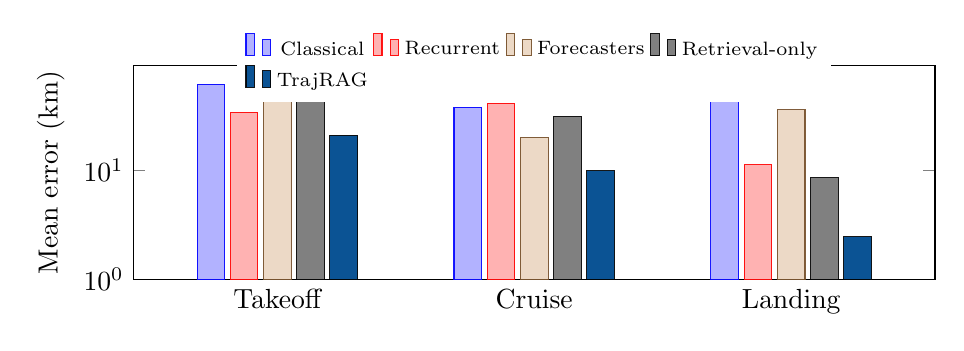
\begin{tikzpicture}
\begin{axis}[
  ybar, width=0.97\linewidth, height=4.3cm,
  ymode=log, log origin=infty,
  bar width=10pt,
  symbolic x coords={Takeoff,Cruise,Landing},
  xtick=data, tick align=inside,
  ylabel={Mean error (km)},
  ymin=1, ymax=90,
  enlarge x limits=0.28,
  legend style={font=\scriptsize, at={(0.5,1.18)}, anchor=north, legend columns=4, draw=none},
  every axis plot/.append style={draw opacity=0.9},
]
\addplot coordinates {(Takeoff,60.95) (Cruise,37.69) (Landing,73.82)};
\addplot coordinates {(Takeoff,33.78) (Cruise,40.66) (Landing,11.17)};
\addplot coordinates {(Takeoff,43.99) (Cruise,19.79) (Landing,35.47)};
\addplot coordinates {(Takeoff,48.94) (Cruise,30.80) (Landing,8.52)};
\addplot[fill=hl] coordinates {(Takeoff,20.78) (Cruise,9.84) (Landing,2.46)};
\legend{Classical,Recurrent,Forecasters,Retrieval-only,TrajRAG}
\end{axis}
\end{tikzpicture}
\end{center}

Four component-level findings from the conference study's ablations carry
over directly to the shared engine used here (numeric per-component table:
conference paper, not reproduced in the journal extension):
\begin{itemize}[leftmargin=14pt, itemsep=1pt, topsep=2pt]
\item \textbf{Removing retrieval caused the largest accuracy degradation in every phase} --- the same component that maritime's own ablation (page 2) identifies as its dominant contributor.
\item \textbf{Replacing the LLM with plain neighbour averaging was significantly worse} --- confirms the gain is not retrieval alone, mirroring the maritime Mean-Retrieval comparison.
\item \textbf{The kinematic feasibility guard mainly reduced variance and worst-case error}, with a smaller effect on the mean --- unlike maritime, where the guard also moves the mean in at least one phase (a genuine cross-domain difference).
\item \textbf{Mixing several routes into one shared memory changed mean error by less than 1\,km} --- memories generalise across routes without a meaningful accuracy cost, supporting the one-service-many-corridors deployment model.
\end{itemize}

\end{document}
